% For generating graphs, mostly waveforms

\documentclass
[varwidth, convert={density=1024, size=1024x768, outext=.png}]
{standalone}

%\documentclass{article}

\usepackage{libertine}

\usepackage[libertine]{newtxmath}

\usepackage{tikz}

\begin{document}

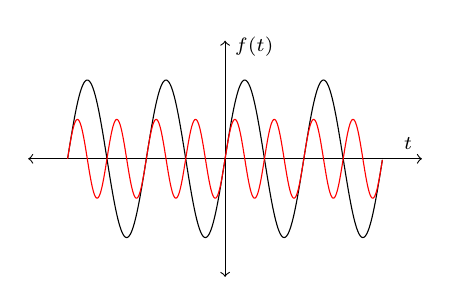
\begin{tikzpicture}[font=\scriptsize]

	% x axis
	\draw [<->]
	      (-2.5, 0) 
	   -- (2.5, 0) node [pos=0.965, above] {$t$};

	% y axis
	\draw [<->] 
	      (0, -1.5) 
	   -- (0,  1.5) node [pos=0.975, right] {$f(t)$};

    \draw [domain=-2:2, samples=1000]
          plot(\x, {sin(2 * pi * \x r)});

    \draw [domain=-2:2, samples=1000, red]
          plot(\x, {0.5 * sin(4 * pi * \x r)});

\end{tikzpicture}

\par $$\Downarrow$$ \par

\iffalse

\begin{tikzpicture}
	% Just for scaling the "graph"
	\draw (0, -1.5) (0, 1.5);

	% The arrow
	\draw (0, 0) node {$\,$\hspace{0.5cm}$\Rightarrow$\hspace{0.5cm}$\,$};
\end{tikzpicture}

\fi

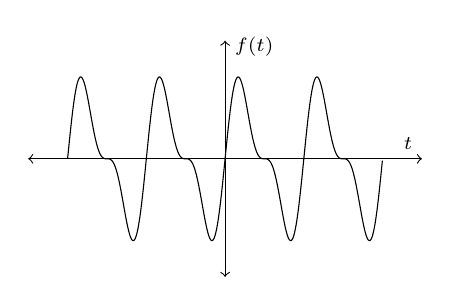
\begin{tikzpicture}

	\tikzstyle{every node}=[font=\scriptsize]

	% x axis
	\draw [<->]
	      (-2.5, 0) 
	   -- (2.5, 0) node [pos=0.965, above] {$t$};

	% y axis
	\draw [<->] 
	      (0, -1.5) 
	   -- (0,  1.5) node [pos=0.975, right] {$f(t)$};

    \draw [domain=-2:2, samples=1000]
          plot(\x, {0.8 * (sin(2 * pi * \x r) + 0.5 * sin(4 * pi * \x r))});

\end{tikzpicture}

\iffalse

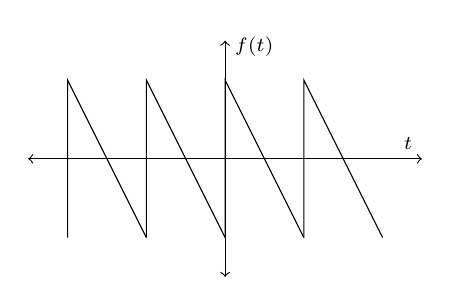
\begin{tikzpicture}

	\tikzstyle{every node}=[font=\scriptsize]

	% x axis
	\draw [<->]
	      (-2.5, 0) 
	   -- (2.5, 0) node [pos=0.965, above] {$t$};

	% y axis
	\draw [<->] 
	      (0, -1.5) 
	   -- (0,  1.5) node [pos=0.975, right] {$f(t)$};

    \foreach \i in {-2, -1, 0, 1} 
    {
    	\draw (\i, -1) -- (\i, 1) -- (\i + 1, -1);
    }

\end{tikzpicture}

\fi

\end{document}